\section{相干种子区：为什么输出可以重复}\label{sec:mechanism}

储备池计算要求同样的输入给出同样的输出，即一致性或回声状态性质~\cite{jaeger2001,uchida2004}，否则训练好的读出层换一次运行就失效。
文献中的单泵浦方案里，梳齿要么由调制不稳定性从噪声中长出来~\cite{shishavan2025}，要么依赖预先建立的孤子态~\cite{cuevas2025,arabieh2026soliton}。
前者的输出取决于起振时的噪声，后者需要把器件稳定在孤子存在区间内。
用谱相位掩模时，输入梳齿本身就落在谐振上，其余梳齿由它们经四波混频产生，是由输入相干地“种”下去的，而不是从噪声中长出来，
这与脉冲或光梳驱动的 Kerr 腔类似~\cite{obrzud2017}。

\subsection{两次运行的比较}

图~\ref{fig:two-runs} 把同一个输入序列送进同一个器件两次，两次运行只有初始的腔内噪声不同。
（a）是原始混沌光梳方案的参数（单个连续泵浦，$325~\mathrm{mW}$，总品质因数 $10^{7}$，归一化失谐约 5；这个点在我们随机搜索的失谐范围之外，见第~\ref{sec:encodings-def}~节）：
由调制不稳定性产生的第 3 根梳齿在两次运行中完全不同，相关系数只有 $0.08$，用这样的特征训练读出层，换一次运行后 NMSE 约为 1。
（b）（c）是一个谱相位掩模的工作点（第~\ref{sec:noise}~节噪声下限研究中选出的点，$23~\mathrm{mW}$，总品质因数 $6\times10^{6}$）。
对输入梳齿（$\mu=3$，图 b），两次重合是意料之中的，因为它被直接驱动；真正的检验是只靠四波混频产生的梳齿（$\mu=12$，图 c，在输入梳齿 $|\mu|\le8$ 之外）。
它的两次运行同样重合，相关系数为 $1.00$，功率比输入梳齿低约十倍。

\begin{figure}[htbp]
\centering
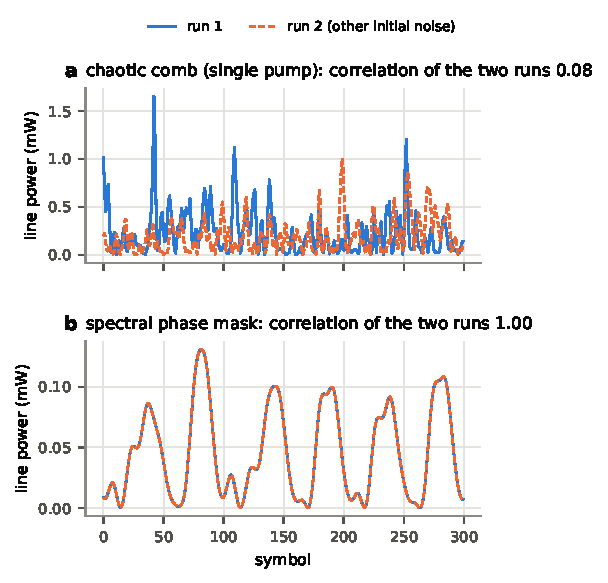
\includegraphics[width=0.8\linewidth]{fig3_two_runs}
\caption{同一输入序列送入同一器件两次，两次运行只有初始的腔内噪声不同（实线和虚线），画出下载端口的梳齿功率（前 300 个符号，不加其他噪声）。
（a）原始混沌光梳方案的参数（单个连续泵浦，$325~\mathrm{mW}$，总品质因数 $10^{7}$，归一化失谐约 5），产生的梳齿 $\mu=3$：相关系数 $0.08$。
（b）（c）谱相位掩模的一个工作点（$23~\mathrm{mW}$，总品质因数 $6\times10^{6}$）：（b）输入梳齿 $\mu=3$，（c）只靠四波混频产生的梳齿 $\mu=12$；相关系数都是 $1.00$。注意纵轴量级不同。}
\label{fig:two-runs}
\end{figure}

\subsection{工作区图}

可重复性只在一定的参数范围内成立。图~\ref{fig:operating-map} 以表~\ref{tab:encodings} 中现实噪声下 Mackey--Glass 选出的掩模工作点为中心，
保持其失谐、调制深度、功率分配和掩模不变，只扫描输入耦合品质因数 $\Qone$（$10^{5.6}$ 到 $10^{7.6}$）和总输入功率（$3$ 到 $1000~\mathrm{mW}$），各取 17 档。
每个格点只用一条序列、一对运行评估，所以是单次噪声实现的值（图中最好的误差 $1.8\times10^{-6}$ 和 $3.3\times10^{-4}$ 恰好舍入后与表~\ref{tab:encodings} 相同）。

无噪声时，74\% 的点一致性高于 $0.99$，是相干种子区。不一致的点（一致性低于 $0.5$，占 16\%）在图~\ref{fig:operating-map}a 实线等值线之外，处于高功率、高 $Q$ 区
（最高 $Q$ 处约 $150~\mathrm{mW}$ 以上，$\Qone\approx2\times10^{6}$ 处约 $1~\mathrm{W}$ 以上），那里调制不稳定性压过输入的种子，光梳回到混沌。
误差在失去一致性之前就已经升高（两条等值线之间），所以高误差和不一致不是一回事。
误差最小的区域在相干种子区内部、靠近混沌区的一侧：误差在最好值 3 倍以内的点都落在 $6$ 到 $79~\mathrm{mW}$、$\Qone=10^{6.1}$ 到 $10^{6.85}$ 之间，
符合“非线性越强越有用，直到失去可重复性”的一般经验。

现实噪声下多出第三个区域。功率太低时，许多梳齿到达探测器的光与探测器噪声相当，读数被淹没，一致性同样下降（图~\ref{fig:operating-map}b 下方虚线以下）；
一致性高于 $0.99$ 的点从 74\% 降到 29\%。可用的点被夹在两者之间：误差在最好值 3 倍以内的点在功率--$Q$ 平面上连成一条斜带（$9$ 到 $336~\mathrm{mW}$），
随 $Q$ 升高向低功率方向倾斜，因为 $Q$ 越高，产生同样非线性所需的功率越低。混沌区在有噪声和无噪声时位置基本相同，因为它的成因（调制不稳定性的增益超过输入种子）与噪声无关。

\begin{figure}[htbp]
\centering
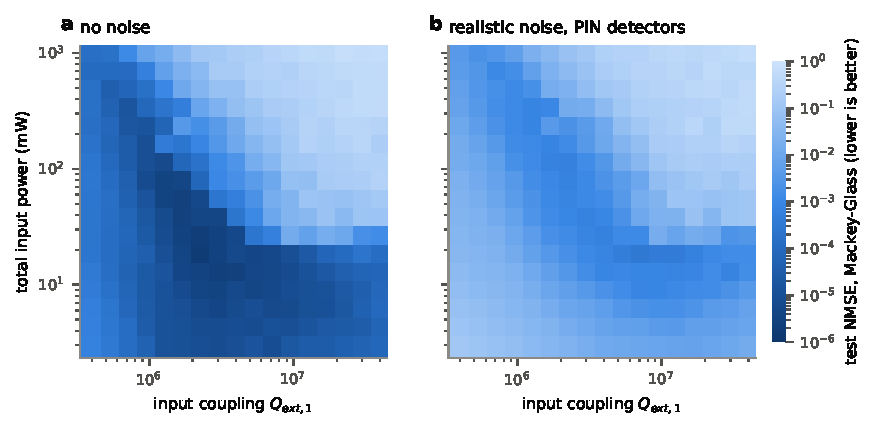
\includegraphics[width=\linewidth]{fig2_operating_map}
\caption{谱相位掩模在表~\ref{tab:encodings} 工作点附近的工作区图（Mackey--Glass，一条序列，每个格点一对运行）。固定其余参数，扫描输入耦合品质因数 $\Qone$ 和总输入功率（各 17 档），
颜色为测试误差（越深越好）。虚线和实线：两次运行一致性为 $0.99$ 和 $0.5$ 的等值线；星号：误差最小点。
（a）无噪声：实线之外（高功率、高 $Q$）是不可重复的混沌区。（b）现实噪声、PIN 探测器：下方虚线以下读数被探测器噪声淹没，可用点在两区之间连成一条带。}
\label{fig:operating-map}
\end{figure}

这一节的结论在后面反复用到：谱相位掩模工作在相干种子、可重复的区域，它的误差来自噪声，而不是不可重复的动力学。
去掉 Kerr 项的对照（第~\ref{sec:linear}~节）表明，掩模在 Mackey--Glass 上的好处主要来自 Kerr 动力学，在信道均衡上则不是：
那里相互干涉的输入梳齿经平方律探测就已提供所需的非线性。
